\section{Description}
The product can be logically divided into two applications -- server side  and client side.
Each application will be used by different kind users and for better distinguishing of all terms we feel need to define them.

\section{Definitions}
%In this section there will be defined and described actors in requirements to avoid misunderstandings. Since our customer namely specified the domain that we should focus on we named the actors as follows.

%\paragraph{User} is a participant of concert who wants to actively take part in show and he can download client application.

%\paragraph{Concert Manager} or simply \textbf{Manager} is a person who controls what media should be played on screen made from mobile phone's of users. 
%He can also manage other general settings.

%\paragraph{Client} or \textbf{Client side} is an application controlled by user and provides him opportunity to be part of the screen by displaying figures on his mobile.

%\paragraph{Server} or \textbf{Server side} is and application controlled by manager and provides him opportunity to change the media displayed on screen.

\begin{figure}[!h]
    \begin{center}
    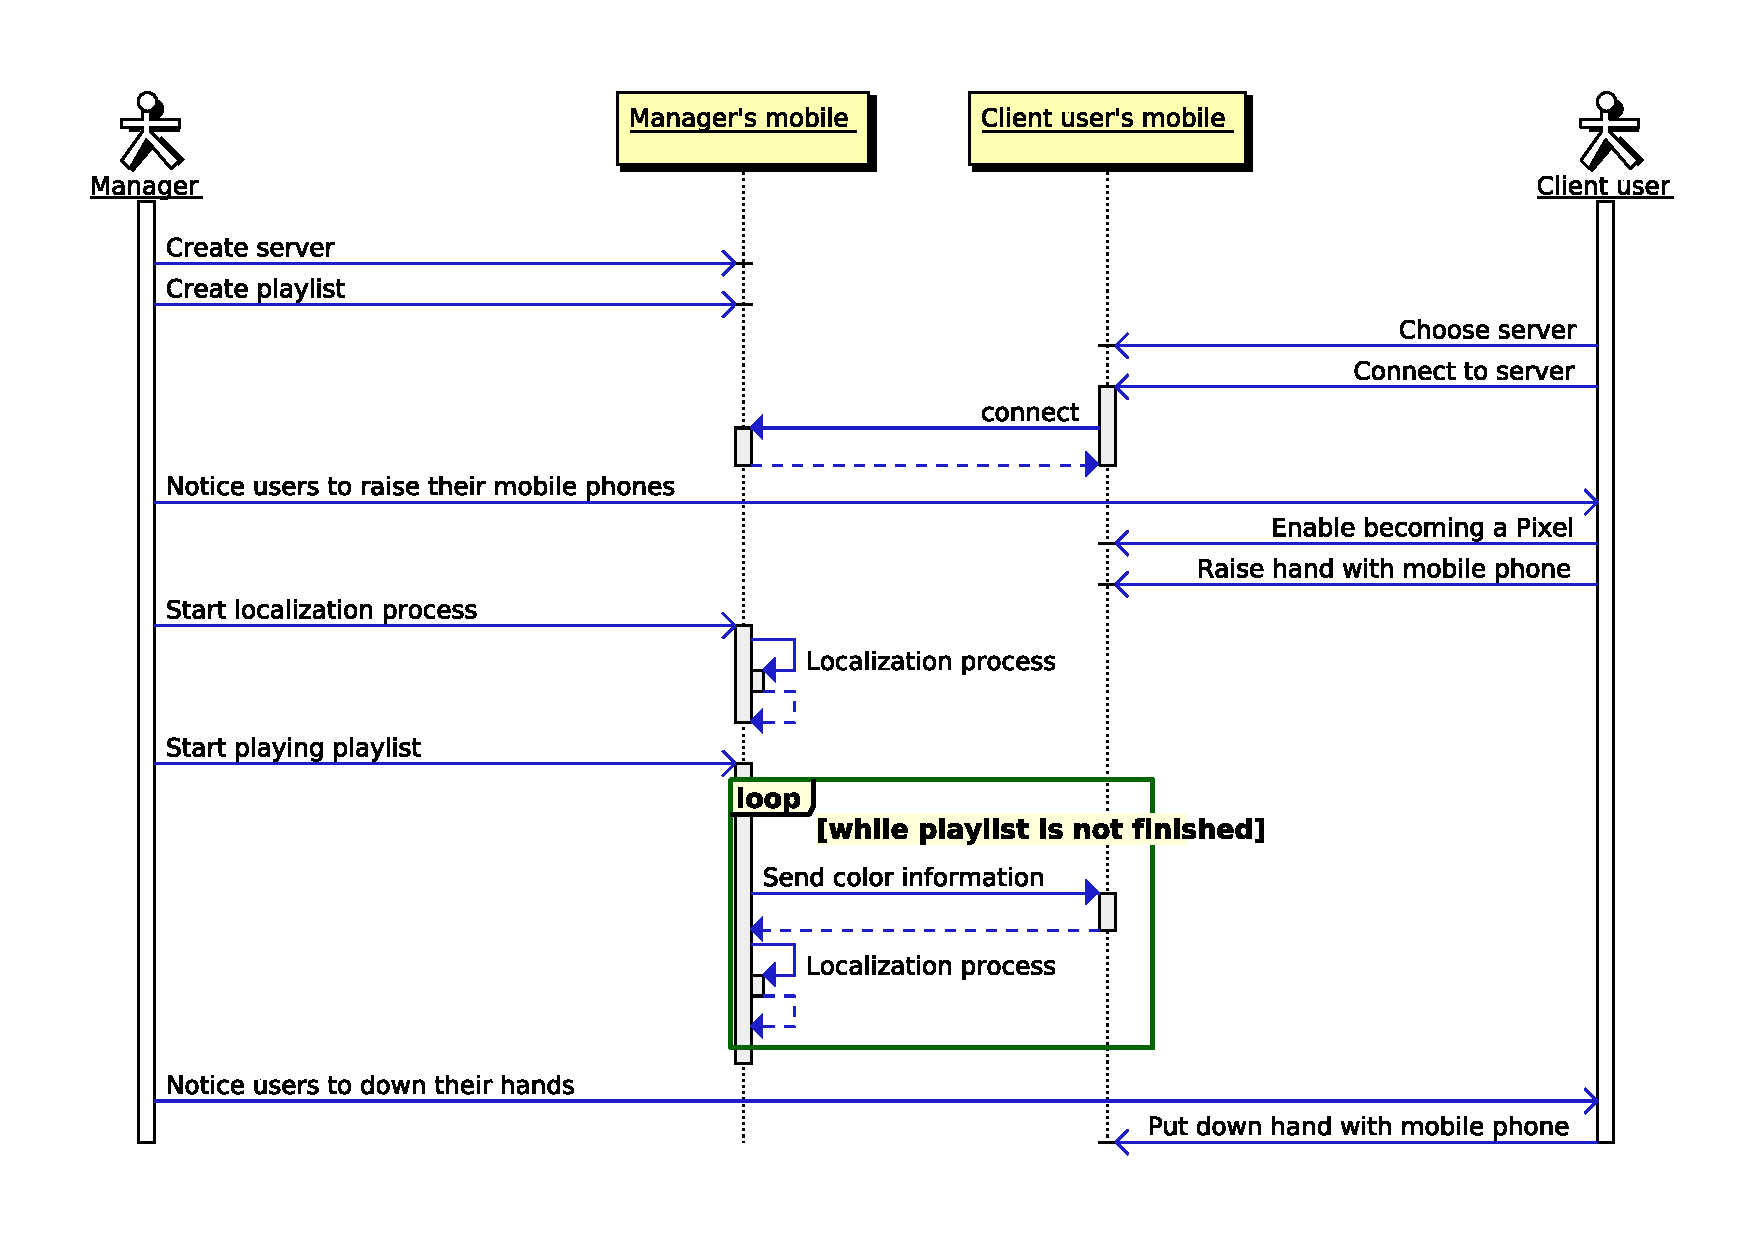
\includegraphics[scale=0.4]{images/wholeapp_seq.pdf}
    \caption{Sequential diagram depicting basic scenario of using product with all actors.}
    \label{img:usecase}
    \end{center}
\end{figure}


\section{Use case diagram}
As we have defined terminology in section \ref{sec:terminology} we will use actor's names according to that terminology.
In the figure bellow is shown use case diagram \ref{img:usecase} of the whole system.

\begin{figure}[!h]
    \begin{center}
    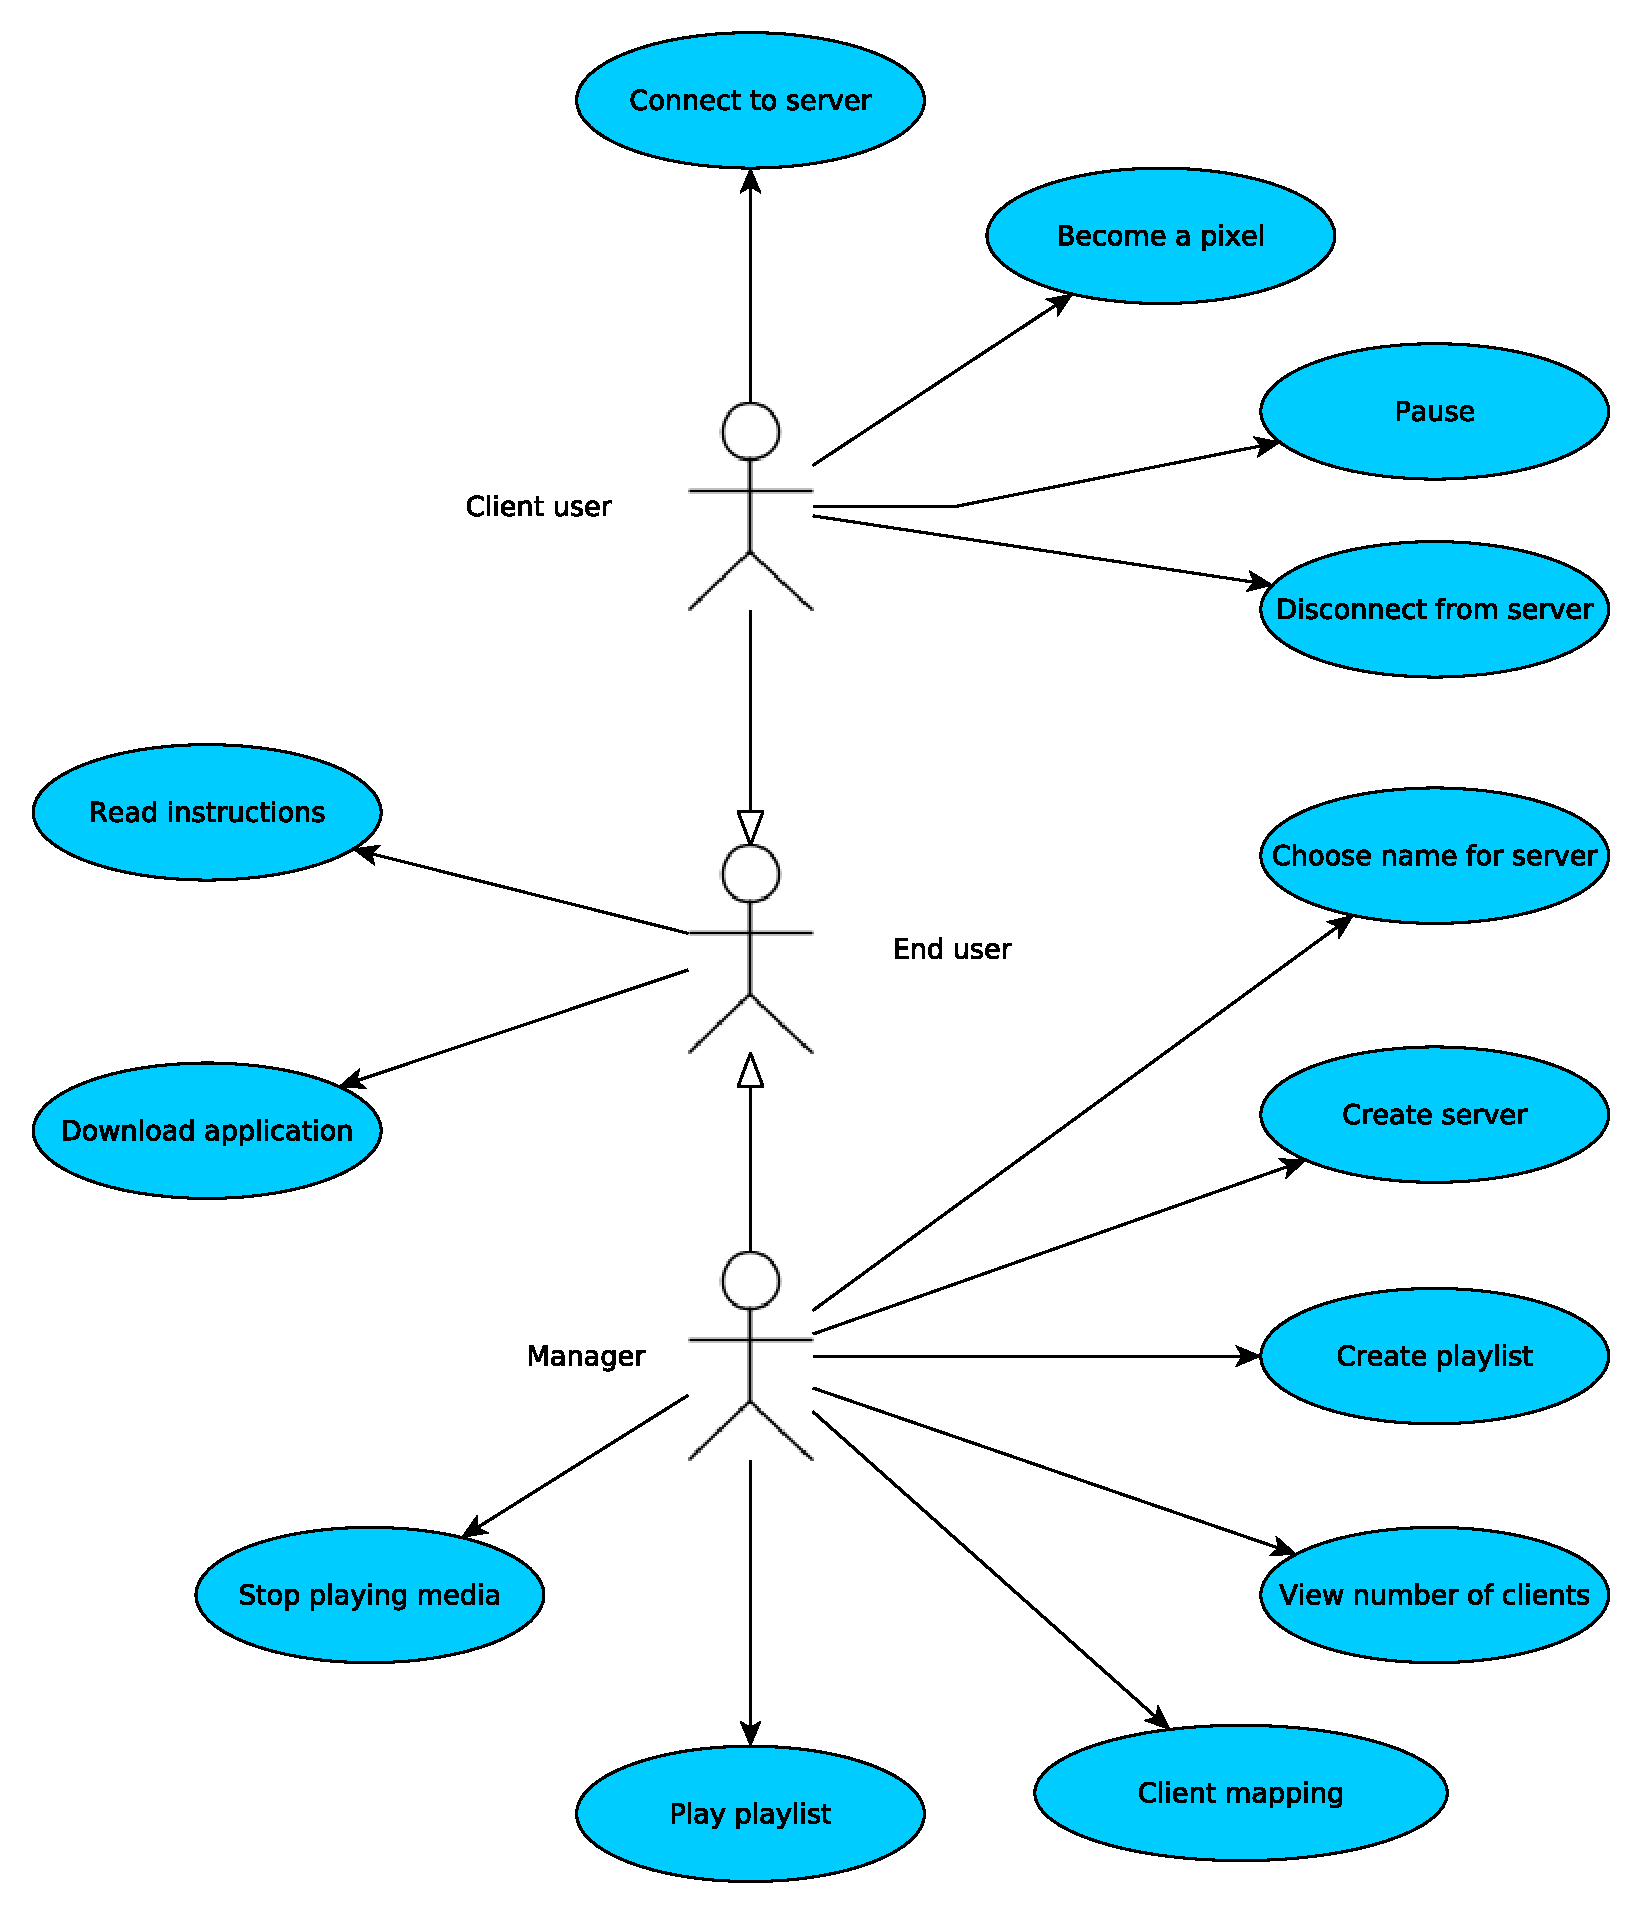
\includegraphics[scale=0.4]{images/usecase.pdf}
    \caption{Use case diagram depicting all actors.}
    \label{img:usecase}
    \end{center}
\end{figure}

\section{Requirements}
According to use case diagram \ref{img:usecase}, requirements were created.


\subsection{Functional}
You can see list of functional requirements from end user's point of view below.
\begin{enumerate}
	\item[\textbf{E1}] \label{req_E1}
		I as a end user want to be able to read instructions.
		
	\item[\textbf{E2}] \label{req_E2}
		I as a end user want to be able to download relevant application from mobile application store.
\end{enumerate}
You can see list of functional requirements from client user's point of view below.
\begin{enumerate}
	\item[\textbf{C1}] \label{req_C1}
		I as a client user I want to easily choose to which server/concert stage I would like to connect.
		
	\item[\textbf{C2}] \label{req_C2}
		I as a client user I want to connect to chosen server.
		
	\item[\textbf{C3}] \label{req_C3}
		I as a client user I want to become a \emph{Pixel}.
	
	\item[\textbf{C4}] \label{req_C4}
		I as a client user I want to be able to pause being a Pixel.
		
	\item[\textbf{C5}] \label{req_C5}
		I as a client user I want to be able to disconnect from server/stage.
\end{enumerate}
You can see list of functional requirements from manager's point of view below.
\begin{enumerate}
	\item[\textbf{M1}] \label{req_M1}
		I as a manager I want to be able to choose name for my server/stage.
		
	\item[\textbf{M2}] \label{req_M2}
		I as a manager I want to be able to create a server.
		
	\item[\textbf{M3}] \label{req_M3}
		I as a manager I want to be able view attendance.
	
	\item[\textbf{M4}] \label{req_M4}
		I as a manager I want to be able to start mobile phone localization.
		
	\item[\textbf{M5}] \label{req_M5}
		I as a manager I want to be able to choose playlist to be played.
		
	\item[\textbf{M6}] \label{req_M6}
		I as a manager I want to be able to start playing given media.
		
	\item[\textbf{M7}] \label{req_M7}
		I as a manager I want to be able to start pause playing the media.
	\item[\textbf{M8}] \label{req_M8}
		I as a manager I want to be able to start pause stop the media.
\end{enumerate}
	
\refreq{E2}


\subsection{Non-functional}
You can see non-functional requirements in table \ref{tab:req_nonfunc}.

\begin{table*}[!h]\centering
\caption{List of all chapters and short description. }
\label{tab:req_nonfunc}
\def\arraystretch{1.3}
\begin{tabularx}{\textwidth}{llX}
\toprule[1mm]
\textbf{ID} & Name & Description\\
\midrule
\textbf{N1} & Server-client architecture & Application must work as a server and client architecture.\\
\textbf{N2} & Platform & Audience application must work on at least one mobile platform.\\
\textbf{N3} & Deployment & Application must be deployed to relevant mobile application store.\\
\textbf{N4} & Scalability & The application must be scalable - it must work with different count of mobile phones.\\
\textbf{N5} & Generality & The application must be prepared for future using outside of rock concert domain.\\
\textbf{N6} & Delivery & Final product must be finished until 21st of November 2013 and presented to the committee and the customer.\\
\bottomrule[1mm]

\end{tabularx}
\end{table*}

\begin{table*}[!h]
	\def\arraystretch{1.25}
	\caption{User stories selected for Sprint 0. }
	\label{tab:usecase1}
	
	\begin{tabular}{p{\textwidth}}
		\toprule[1mm]
		\textbf{Use case detail: Create playlist} \\
		\midrule	
		Actors: Manager \\
		Conditions:
		
		\begin{enumerate}
			\item Manager had created server.
		\end{enumerate}
		\\
		\bottomrule[1mm]
	\end{tabular}
\end{table*}

\section{Summary}
